\begin{center}
    \Large{\textbf{第四章“一维定态问题”题目参考答案}}
\end{center}

本章作业题的解答请主要参考张鹏飞《习题解答》,本文档就部分题目提供一些额外的解法与讨论。文档最后是习题课上所讲的几道例题,供同学们参考。

另外习题课上的MMA演示已放在“习题课资料”文件夹下(之后还会更新),也推荐大家关注~\url{https://demonstrations.wolfram.com/},上面有很多量子力学相关的MMA演示,是很棒的辅助学习资料。


\begin{enumerate}[label=\textbf{4.\arabic*}, listparindent=\parindent]

\setcounter{enumi}{0}
\item 《解答》中给出的是更具有普适性的证法,对任意空间(包括任意维度希尔伯特空间、描述自旋的复欧式空间等等)都是适用的。还有另一个常用的证法,在这里以一维希尔伯特空间为例:

设$\psi_1(x)$, $\psi_2(x)$分别为能量本征值$E_1$, $E_2$的本征波函数,则有
\[-\frac{\hbar^2}{2m}\dv[2]{x}\psi_i(x) + V(x)\psi_i(x)=E_i\psi_i(x),\quad \text{$i=1,2$ 记为(1),(2)式}\]
计算$\psi_2^*\times(1)-\psi_1\times(2)^*$并对$x$无穷积分有
\[\intif \qty(\psi_2^*\dv[2]{\psi_1}{x}-\psi_1\dv[2]{\psi_2^*}{x})\dd{x} = (E_1-E_2)\intif\psi_2^*\psi_1\dd{x}.\]
由于
\[\psi_2^*\dv[2]{\psi_1}{x}-\psi_1\dv[2]{\psi_2^*}{x} = \dv{x}\qty(\psi_2^*\psi_1' - \psi_1\psi_2'^*),\]
所以积分的左式变为$\eval{\psi_2^*\psi_1' - \psi_1\psi_2'^*}_{-\infty}^\infty$,对束缚态有$x\rightarrow \pm\infty$时$\psi\rightarrow 0$,故该式为0,又因为$E_1\neq E_2$,故
\[\intif\psi_2^*\psi_1\dd{x} =0\]
即两个量子态正交。

\noindent\textbf{\color{red}讨论:}事实上,以上的解法与《解答》的解法看似不同,{\color{red}其本质却是一样的。}《解答》中用到了$\hat{H}$是厄米算符的性质,于是直接写出了$(\psi_2,\,\hat{H}\psi_1)=(\hat{H}\psi_2,\,\psi_1)$。而上面的过程中相当于把$\hat{H}$是厄米算符的性质重新证明了一遍。事实上,证明$\im\dv{x}$, $\dv[2]{x}$这类算符是厄米算符过程中的“关键步骤”正是将$x$上的无穷积分转化为边界上的值,也即类似于“分部积分”的思想,这与上面的过程是一样的。

\setcounter{enumi}{4}
\item
本题有另一种化简形式,动量空间波函数可写作
\[\varphi_n(p) = \sqrt{\frac{n^2\pi \hbar^3}{a^3}}\frac{1}{p^2 - (n\pi\hbar/a)^2}\qty((-1)^n \ee{-\im pa/\hbar} - 1),\]
动量概率密度幅为
\[|\varphi_n(p)|^2 = \frac{2n^2\pi \hbar^3}{a^3}\frac{1}{\qty(p^2 - (n\pi\hbar/a)^2)^2}\qty(1-(-1)^n\cos(\frac{pa}{\hbar})).\]
由分母的形式,也容易分析出整数$n$确定时$|\varphi_n(p)|^2$在$p = \pm n\pi\hbar/a$时取得极大,$n$很大时函数图像呈现出相互分离的两个峰。

\noindent\textbf{\color{red}讨论:}《解答》最后提到了泡利与朗道就无限深方势阱中粒子动量分布的争论的典故。其核心问题在于,从局域的角度理解看势阱中是精确的“驻波”解,动量应当只有确定的取值,这与本题量子力学给出的推断不符。文中提到的两本《量子力学》文献已放入网盘“作业解答”文件夹,感兴趣的同学可以自行阅读思考。

\setcounter{enumi}{8}
\item 
\noindent\textbf{\color{red}讨论:}我们还可以讨论一个有趣的问题:量子力学的无限深方势阱模型是如何向经典情形下小球在两壁间往返运动过渡的?

对非定态波函数在势阱中运动的情形,《解答》中“说明4”告诉我们,因为有不同定态之间“干涉项”的存在,两壁的瞬时作用力并不相等。我们可继续通过计算表明,其作用力随时间虽然会发生变化,但“干涉项”所导致的作用力的分量随时间平均一定为0.

下面作一般的讨论。考虑波函数为定态波函数的线性组合
\[\psi(x) = \sum_{n}C_n \Psi_n(x),\]
对于给定区间$[x_1,\,x_2]$的作用力算符,可由势能算符定义为
\[\hat{F} = \begin{cases}
-\dv{V(x)}{x},& x\in [x_1,\,x_2]\\
0,&\text{其他}
\end{cases}\]
在本题中右壁给粒子作用力为$F(x) = -V_0\,\delta(x-\frac{a}{2})$.
于是在$[x_1,\,x_2]$区间内粒子所受作用力为
\alg{\langle F\rangle &= \intif \psi^*(x)F(x)\psi(x) \dd{x}\\
& = \sum_n \abs{C_n}^2\intif \Psi_n^*(x)F(x)\Psi_n(x)\dd{x} + \sum_{m,n} C_m^*C_n \intif \Psi_m^*(x)F(x)\Psi_n(x)\dd{x}}
考虑上式在长时间下的平均。显然,第一项为定态波函数的受力,不随时间变化;第二项为干涉项,不难发现它是$t$的周期函数,其$n,m$项在长时间下的平均可计算为:
\alg{\overline{\langle F\rangle}_{m,n}& = 
\frac{1}{2\pi\hbar/(E_m-E_n)}\int_0^{\frac{2\pi\hbar}{E_m-E_n}}\dd{t}\qty(
C_m^*C_n\ee{\im \frac{E_m t}{\hbar}}\ee{-\im \frac{E_n t}{\hbar}} \intif \Psi_m^*(x)F(x)\Psi_n(x)\dd{x})=0}
因此在长时间平均下只有定态项贡献作用力,也即
\[\overline{\langle F\rangle} = \sum_n \abs{C_n}^2\intif \Psi_n^*(x)F(x)\Psi_n(x)\dd{x} = \sum_n \abs{C_n}^2 F_n\]

势阱下粒子运动的经典模型为小球在两壁间不断反弹,动能只取$\pm p_\mathrm{cl}$。量子情形向经典的过渡应为{\color{red}一个很窄的波包在两壁间不断运动并反弹,且在缓慢地扩散}。显然,在经典尺度下势阱宽度$a$应当很大,波包能量应有$E_\mathrm{cl}\gg E_0$, $E_0$为基态能量。该波包波函数可在本征波函数组$\{\Psi_n\}$下展开,其非零系数应主要集中在$E_\mathrm{cl} = p_\mathrm{cl}^2/2m$定态的附近,其宽度$\Delta E_\mathrm{cl}$应有$\Delta E_\mathrm{cl}\ll E_\mathrm{cl}$。

对$E_\mathrm{cl}$附近很窄区域内的各定态,它们单独存在时右壁提供的作用力是恒力,$F_n \approx -E_\mathrm{cl}/a$。根据上面的受力公式,波包受右壁的平均作用力是各个定态分量所受作用力以概率为权重的加权平均,即
\[\overline{\langle F\rangle} \approx -E_\mathrm{cl}/a\]
与经典情形相同。

以上论证了平均受力是相同的,还可以论证$\overline{\langle F\rangle}$随时间的变化模式也是相同的。根据解答已知,对作用力$F(x) = -V_0\;\delta(x-\frac{a}{2})$,任意瞬时波函数$\psi(x)$(已归一化)受到右壁提供的力为$\langle F\rangle = -V_0\abs{\psi(\frac{a}{2})}^2$。各定态单独存在时,右壁提供的力是恒定不变的;而对于波包的情形,在波包冲向右壁或远离右壁过程中,$x=\frac{a}{2}$处波函数值非常小,故受力几乎为0,而在波包达到右壁发生反弹的过程中,可以预见$x=\frac{a}{2}$处波函数值较大,受力应当较大。这与经典情形也是相同的。

\setcounter{enumi}{11}
\item (不要求)

题目推导稍微有误。按照$\psi = \xi^{-\im k_2 a}u(\xi)$的代换方式,并不能使得$u(\xi)$在$\xi\rightarrow 0$ (即$x\rightarrow+\infty$)时趋于常数。若要做到这一点,应作代换
\[\psi = \xi^{-\im k_1 a}u(\xi)\]
后续的推导过程相仿,最后得到$u(\xi)$的方程为
\[\xi(1-\xi)u''+(2-\im k_1 a)(1-\xi)u'-(k_2^2-k_1^2)a^2 u =0\]
解得两个合流超几何函数解:$u_1 = \mathrm{F}(\alpha,\,\beta,\,\gamma,\,\xi)$, $u_2 = \xi^{1-\gamma}\mathrm{F}(\alpha-\gamma+1,\,\beta-\gamma+1,\,2-\gamma,\,\xi)$,其参数为
\[\begin{cases}
\alpha = -\im(k_2+k_1)a\\
\beta = \im(k_2-k_1)a\\
\gamma = -2\im k_1 a+1
\end{cases}\]
考虑边界条件为$\xi\rightarrow 0$时$u(\xi)$有限,故应选取$u_1$解。但请注意$u_2$解并不是因“非物理”的缘故而将其舍去的,它也是一个合理的波函数。舍去的原因是,它在$\xi\rightarrow 0$ (即$x\rightarrow+\infty$)时有$\psi\sim \xi^{\im k_1 a}\sim \ee{-\im k_1 x}$,这是沿反方向入射的波,不是本题考虑的对象。不过也请注意,$u_2$解并不是沿$-x$方向入射的波经势场反射、透射后形成的波函数,因为这一波函数在$x\rightarrow +\infty$同时有沿$\pm x$方向传播的成分。可以理解为$u_2$解是这一波函数与$u_1$解的一个线性叠加。

\setcounter{enumi}{12}
\item
\noindent\textbf{\color{red}讨论:相速、群速的原理复习。}

首先考虑一系列波矢为$k$的同向波的叠加,它们各自有相位$\theta(k)$。若$k=k_0$波的成分最大(即在$k$表象上波函数为中心在$k=k_0$处的波包),问在$x$表象上将在哪里形成波包?

为此写出普适的$x$表象波函数:
\[\psi(x) = \intif A(k)\ee{\im k x-\theta(k)}\dd{k}\]
这里$A(k)$为实数,因相位都被吸收进$\theta(k)$里面了。显然$k=k_0$分量应对波函数形状影响最大。当$k$在$k_0$附近微小变化时,若存在某点$x_0$使不同$k$值的波的相位相同,则该点处应当叠加地最猛烈,对应$x$表象波包中心。因此
$x_0$满足\[\eval{\dv{k}\qty(k x_0+\theta(k))}_{k=k_0} = 0\]
\[x_0 = \eval{\dv{\theta(k)}{k}}_{k=k_0}.\]
注意上面只是一个合理的估计,并不是严格的推导。波函数严格的极大值点显然与$A(k)$形式有关系,实际结果应相比上式有微小偏差。对该式的一个简单验证时是高斯波包:令$A(k)\sim \ee{-\alpha^2(k-k_0)^2}$, $\theta(k) = kx_0$,在$x$表像可计算出$\psi(x)\sim \ee{-\frac{(x-x_0)^2}{4\alpha^2}}\ee{\im k_0(x-x_0)}$,波包在$x_0$处。

进一步考虑波随时间的演化,出于色散效应每个$k$波有各自的角频率$\omega(k)$,因此每个$k$波的相速度$v_\mathrm{p}=\frac{\omega(k)}{k}$。由于$k=k_0$波的成分显著最大,对整列波的影响最大,故整列波的相速度受其影响为$v_\mathrm{p}=\frac{\omega(k_0)}{k_0}$. 现在波函数为
\[\psi(x) = \intif A(k)\ee{\im k x-\omega(k)t-\theta(k)}\dd{k}\]
按照上面分析,波函数极大值值点此时应为
\[x_0 =  \eval{\dv{\omega(k)}{k}}_{k=k_0}t +  \eval{\dv{\theta(k)}{k}}_{k=k_0}.\]
其移动速度即为群速度$v_\mathrm{g}=\eval{\dv{\omega(k)}{k}}_{k=k_0}$。

\item
(需将《解答》中$V_0$改为$-V_0$)

\setcounter{enumi}{20}
\item
\noindent\textbf{\color{red}讨论:}本题的$V =V_0\qty(\frac{a}{x}-\frac{x}{a})^2 $势能下的能级也呈现等差数列的分布样式,与谐振子特征相同。容易使人想到,这背后是否有更加本质的数学机制来支撑呢?本例中的哈密顿量$\hH$是否也能写成形如$\ha^\dagger\ha$的形式呢?

事实上$\hH$的确可以写成$\ha^\dagger\ha$的形式,但此处不再有$[\ha,\,\ha^\dagger]=1$,于是需要引入一些巧妙的办法处理。不过,本题仅用量子力学的算符方法求解是完全可行的,感兴趣的同学可参考:程檀生《现代量子力学基础》第七章\;因子化方法,重点参考p.~220--222(不作要求)。

\setcounter{enumi}{22}
\item
\noindent\textbf{\color{red}讨论:}本题可在解题前就$p$空间上的波函数形成一些直观感觉。由于$x<0$和$x>0$的势是常量,那么其上的波函数一定是“单色”波函数的一部分,所以转化到$p$空间的谱上一定会出现相应的$\delta$峰,这就是$C_1\,\delta(p-\hbar k)+C_2\,\delta(p+\hbar k)$的来源。


\setcounter{enumi}{25}
\item 【另解】

就入射波经过两层$\delta$势的情形,不妨依次考虑波在每层势垒的透射、反射过程。由单层$V_0=\gamma\delta(x)$势对波的散射规律可知,反射系数$r$与透射系数$s$分别为
\[r = \frac{1}{\im \theta-1},\quad s=\frac{\im\theta}{\im\theta-1},\quad\text{其中$\theta = \frac{\hbar^2 k}{m\gamma}$}\]
在波抵达$\delta$势时会依照上式发生透射、反射,因此波的传播路程如下图所示。其中的复数表示的是相应波前的振幅。
\begin{figure}[!ht]
    \centering
    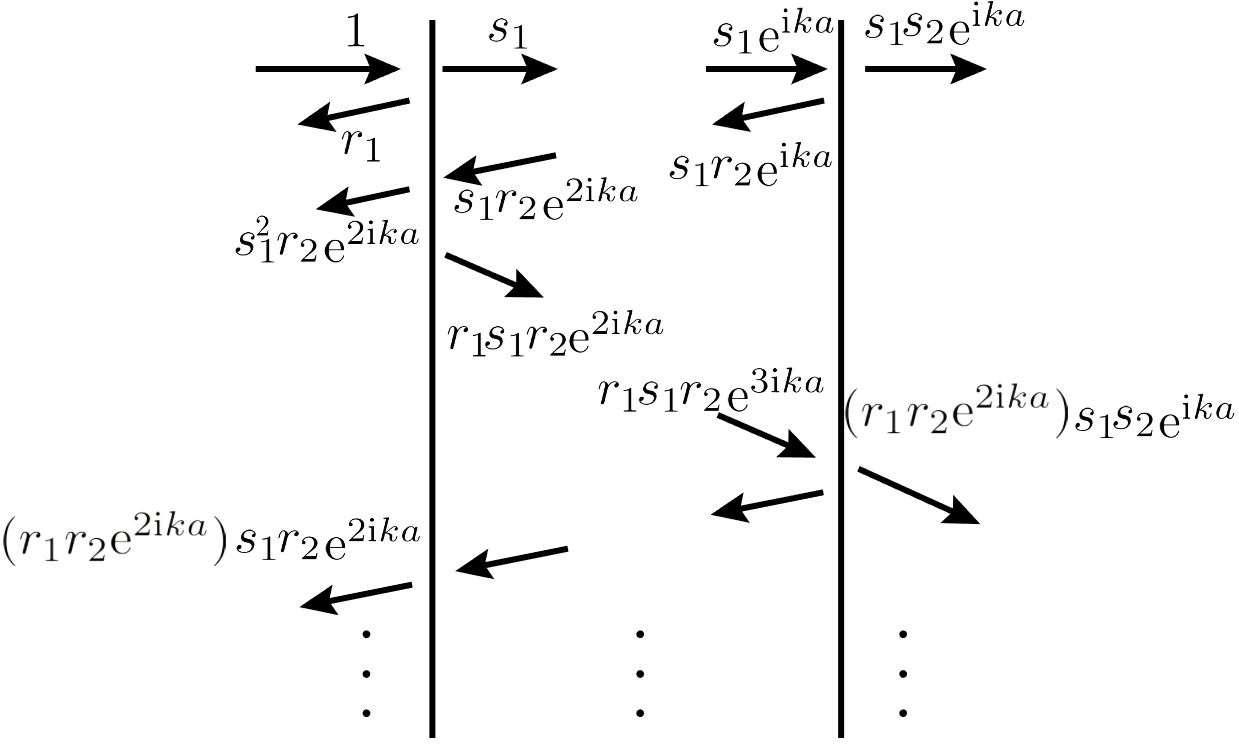
\includegraphics[width=0.5\textwidth]{pic/delta.JPG}
    \label{fig:my_label}
\end{figure}

下面要严格论证的是,将三段区间内的所有波叠加起来,形成的波函数是满足薛定谔方程的;同时因为级数收敛,它是一个合理的解。这是因为在$x=0,\,a$的边界上波函数需满足
\[ \begin{cases}
-\frac{\hbar^2}{2\mu}\qty(\psi'(0^+)-\psi'(0^-))+\gamma_1\psi(0) = 0\\
-\frac{\hbar^2}{2\mu}\qty(\psi'(a^+)-\psi'(a^-))+\gamma_2\psi(a) = 0
\end{cases}\]
而在边界附近可就所有波以“入射、反射、透射”的形式编组,每个组合构成的局域波函数均满足上述方程。由于波函数的叠加性可知道上图即给出一个合理的波函数解。因此,只需统计所有从第1层$\delta$势垒反射回来的波函数即可:
\alg{R &= r_1+s_1^2r_2\ee{2\im ka}\qty(1+r_1r_2\ee{2\im ka}+(r_1r_2\ee{2\im ka})^2+\cdots)\\
&= r_1+s_1^2r_2\ee{2\im ka}\frac{1}{1-r_1r_2\ee{2\im ka}}\\
&= \frac{1}{\im\theta_1 -1}+\frac{-\theta_1^2}{(\im\theta_1 -1)^2}\frac{1}{\im\theta_2 -1}\ee{2\im ka}\frac{(\im\theta_1-1)(\im\theta_2-1)}{(\im\theta_1-1)(\im\theta_2-1)-\ee{2\im ka}}\\
&= \frac{(\im\theta_2-1)+(\im\theta_1+1)\ee{2\im ka}}{(\im\theta_1-1)(\im\theta_2-1)-\ee{2\im ka}}
}
透射系数的计算类似,容易发现结果与《解答》相同。

\item 【另解】

仿照4.26题的方法求解。但此时逐个地对无限层$\delta$势垒写入射波的反射、透射的波函数是不现实的,我们可将所有势垒层看做一个黑箱,且将第2层到$\infty$层势垒视为同样的黑箱。设入射波前振幅为1,经过黑箱后反射系数$u$,透射系数$v$(注意应固定与第一层势垒的距离,相位会随距离变化产生差异),容易绘制出波的传播路径如下。
\begin{figure}[!ht]
    \centering
    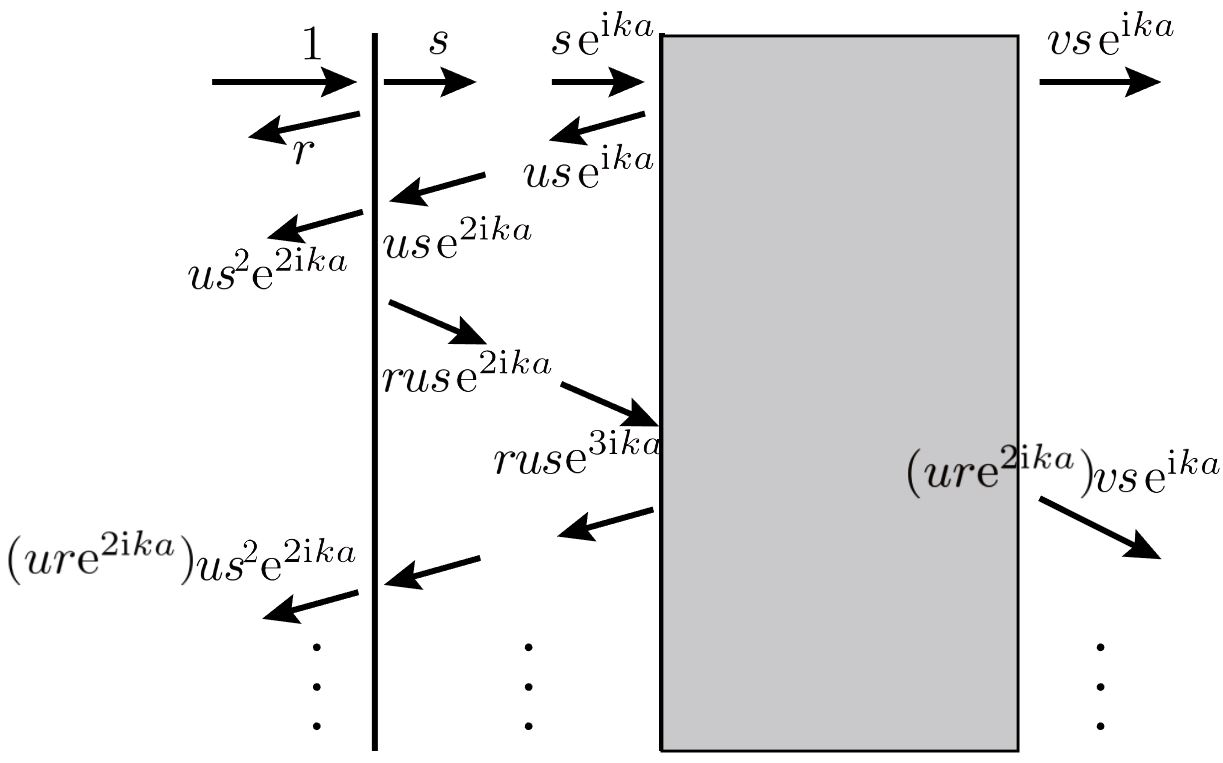
\includegraphics[width=0.5\textwidth]{pic/delta2.JPG}
    \label{fig:my_label}
\end{figure}

经过黑箱的透射波为
\alg{v & = \qty[s\ee{\im ka}\qty(1+ur\ee{2\im ka}+(ur\ee{2\im ka})^2+\cdots)]\,v\,\ee{-\im ka}\\
&= v\,\frac{1+r}{1-ur\ee{2\im ka}}
}
这里用到$s=1+r$. 可得$u\ee{2\im ka}=-1$. 经过黑箱的反射波为
\alg{u &= r+us^2\ee{2\im ka}\qty(1+ur\ee{2\im ka}+(ur\ee{2\im ka})^2+\cdots)\\
&= r+ \frac{u(1+r)^2\ee{2\im ka}}{1-ur\ee{2\im ka}}\\
&= \frac{r+u(1+2r)\ee{2\im ka}}{1-ur\ee{2\im ka}}}
代入$u\ee{2\im ka}=-1$可得$u=-1$,从而$\ee{2\im ka}=1$.

\end{enumerate}

\begin{enumerate}[label=\textbf{4.A\arabic*}, listparindent=\parindent]
    \item (出自《樱井》习题2.12)\textbf{考虑一维谐振子势,若$t=0$时系统处于$\ket{\psi}=\exp(-iAp/\hbar)\ket{0}$态,利用Heisenberg绘景计算$\jkh{x(t)}$和$\jkh{p(t)}$。}\\
    \textbf{解:}首先计算$\zkh{H,\,x}$和$\zkh{H,\,p}$:
    \alg{\zkh{H,\,x}&=\frac{1}{2m}\zkh{p^2,\,x}=-\im\frac{\hbar}{m}p\\
    \zkh{H,\,p}&=\frac{m\omega^2}{2}\zkh{x^2,\,p}=\im\hbar m\omega^2x}
    根据定义,可以写出Heisenberg绘景下坐标算符的表达式:
    \alg{x_\mathrm{H}(t)=\ee{\frac{\im Ht}{\hbar}}x_\mathrm{S}\ee{-\frac{\im Ht}{\hbar}}}
    利用恒等式$\ee{-\alpha\hA}\hB\ee{\alpha\hA}=\sum_{n=0}^\infty\frac{\alpha^n}{n!}(-1)^n(\mathcal{L}_{\hA})^n(\hB)$,可得
    \alg{x_\mathrm{H}(t)&=\sum_{n=0}^\infty\frac{\xkh{\im t/\hbar}^n}{n!}(\mathcal{L}_{H})^n(x_\mathrm{S})\\
    &=\sum_{n=0}^\infty\frac{\xkh{-\omega t}^{2n}}{\xkh{2n}!}x_\mathrm{S}+\frac{1}{m\omega}\sum_{n=0}^\infty\frac{\xkh{-\omega t}^{2n+1}}{\xkh{2n+1}!}p_\mathrm{S}\\
    &=x_\mathrm{S}\cos\omega t+\frac{p_\mathrm{S}}{m\omega}\sin\omega t}
    类似地,可以得到Heisenberg绘景下动量算符的表达式:
    \alg{p_\mathrm{H}(t)=p_\mathrm{S}\cos\omega t-m\omega x_\mathrm{S}\sin\omega t}
    则$t$时刻的$\jkh{x_\mathrm{H}(t)}$为
    \alg{\jkh{x_\mathrm{H}(t)}&=\bra{\psi}x_\mathrm{H}(t)\ket{\psi}\\
    &=\bra{0}\ee{\im\frac{Ap}{\hbar}}x_\mathrm{H}(t)\ee{-\im\frac{Ap}{\hbar}}\ket{0}\\
    &=\bra{0}\xkh{\ee{\im\frac{Ap}{\hbar}}x_\mathrm{S}\ee{-\im\frac{Ap}{\hbar}}\cos\omega t+\frac{1}{m\omega}\ee{\im\frac{Ap}{\hbar}}p_\mathrm{S}\ee{-\im\frac{Ap}{\hbar}}\sin\omega t}\ket{0}\\
    &=\bra{0}\zkh{(x_\mathrm{S}+A)\cos\omega t+\frac{1}{m\omega}p_\mathrm{S}\sin\omega t}\ket{0}\\
    &=A\cos\omega t}
    最后一步可通过将$x$和$p$用升降算符表示得到(易知$\jkh{x}=0$,$\jkh{p}=0$)。类似地,可知
    \alg{\jkh{p_\mathrm{H}(t)}=-Am\omega\sin\omega t}\\
    \textbf{补充:}此系统实际上对应相干态,$t=0$时处在$c$为实数的相干态。下面考察任意相干态的时间演化。考虑相干态
    \alg{\ket{c}=\ee{-\frac{1}{2}\abs{c}^2}\ee{ca\hcj}\ket{0}=\ee{-\frac{1}{2}\abs{c}^2}\sum_0^\infty\frac{c^n}{\sqrt{n!}}\ket{n}}
    由于$\ket{n}$是$H$的本征态,其时间演化只需乘一个相因子,易得
    \alg{\ket{c}(t)&=\ee{-\frac{1}{2}\abs{c}^2}\sum_0^\infty\frac{c^n}{\sqrt{n!}}\ee{-\im\omega t\xkh{n+\frac{1}{2}}}\ket{n}\\
    &=\ee{-\frac{1}{2}\abs{c}^2}\ee{-\frac{1}{2}\im\omega t}\sum_0^\infty\frac{\xkh{c\ee{-\im\omega t}}^n}{\sqrt{n!}}\ket{n}\\
    &=\ee{-\frac{1}{2}\im\omega t}\ket{c\ee{-\im\omega t}}}
    可见相干态在任意$t$时刻仍为相干态。考察$\jkh{x}$和$\jkh{p}$,由于相干态中$\jkh{x}\propto\Re{c}$,$\jkh{p}\propto\Im{c}$,可知$\jkh{x}$和$\jkh{p}$随时间简谐地振荡。这可看作经典谐振子在量子中的对应。
    
    \item(出自《樱井》习题2.18)\textbf{证明一维谐振子势下有}
    \alg{\bra{0}\ee{\im kx}\ket{0}=\exp(-\frac{k^2}{2}\bra{0}x^2\ket{0})}
    \textbf{解:}将$x$用升降算符表示:
    \alg{\ee{\im kx}=\exp(\im k\sqrt{\frac{\hbar}{2m\omega}}\xkh{a+a\hcj})=\exp(\im k\sqrt{\frac{\hbar}{2m\omega}}a\hcj)\exp(\im k\sqrt{\frac{\hbar}{2m\omega}}a)\exp(-\frac{1}{2}k^2\frac{\hbar}{2m\omega})}
    则等式左边可写为:
    \alg{\bra{0}\ee{\im kx}\ket{0}&=\bra{0}\exp(\im k\sqrt{\frac{\hbar}{2m\omega}}a\hcj)\exp(\im k\sqrt{\frac{\hbar}{2m\omega}}a)\exp(-\frac{1}{2}k^2\frac{\hbar}{2m\omega})\ket{0}\\
    &=\exp(-\frac{1}{2}k^2\frac{\hbar}{2m\omega})\bra{0}\exp(\im k\sqrt{\frac{\hbar}{2m\omega}}a\hcj)\ket{0}\\
    &=\exp(-\frac{1}{2}k^2\frac{\hbar}{2m\omega})}
    另一方面,计算$\bra{0}x^2\ket{0}$:
    \alg{\bra{0}x^2\ket{0}=\bra{0}\frac{\hbar}{2m\omega}\xkh{a^2+{a\hcj}^2+aa\hcj+a\hcj a}\ket{0}=\frac{\hbar}{2m\omega}}
    容易看出上式只有$\bra{0}aa\hcj\ket{0}=1$项非0。故有
    \alg{\bra{0}\ee{\im kx}\ket{0}=\exp(-\frac{1}{2}k^2\frac{\hbar}{2m\omega})=\exp(-\frac{1}{2}k^2\bra{0}x^2\ket{0})}
    
    \item(出自《樱井》习题2.16)\textbf{定义关联函数为}
    \alg{C(t)=\jkh{x_\mathrm{H}(t)x_\mathrm{H}(0)}}
    \textbf{计算一维谐振子基态下的$C(t)$。}\\
    利用4.I的结果,有
    \alg{x_\mathrm{H}(t)x_\mathrm{H}(0)=x_\mathrm{S}^2\cos\omega t+\frac{p_\mathrm{S}x_\mathrm{S}}{m\omega}\sin\omega t}
    将$x$和$p$用升降算符表示,有
    \alg{&p\xde x\xde=\im\frac{\hbar}{2}\xkh{-a\xde^2+a\hcj\xde{^2}-1}\\
    &x\xde^2=\frac{\hbar}{2m\omega}\xkh{a\xde{^2}+a\hcj\xde{^2}+a\xde a\hcj\xde+a\hcj\xde a\xde}}
    容易得到
    \alg{&\bra{0}p\xde x\xde\ket{0}=-\im\frac{\hbar}{2}\\
    &\bra{0}x\xde^2\ket{0}=\frac{\hbar}{2m\omega}}
    故
    \alg{C(t)=\frac{\hbar}{2m\omega}\cos\omega t-\im\frac{\hbar}{2m\omega}\sin\omega t=\frac{\hbar}{2m\omega}\ee{-\im\omega t}}

\item (出自程檀生书习题3.13) \textbf{在$xy$平面上运动的质量为$m$,电荷$e$的粒子被置于均匀的磁场中($\vec{B}=B_0\vec{e}_z$),其哈密顿量$\hH$可以表为
\[\hat{H}=\frac{1}{2m}\qty{\hat{p}_x^2+\hat{p}_y^2+eB_0(y\hat{p}_x-x\hat{p}_y)+\frac{1}{4}e^2B_0^2(x^2+y^2)}\]
设\[\hat{b} = \frac{1}{\sqrt{2eB_0 \hbar}}\qty(\frac{1}{2}eB_0x + \im\hat{p}_x+\frac{1}{2}\im eB_0 y-\hat{p}_y),\]
\[\hat{b}^\dagger = \frac{1}{\sqrt{2eB_0 \hbar}}\qty(\frac{1}{2}eB_0x -\im\hat{p}_x-\frac{1}{2}\im eB_0 y-\hat{p}_y),\]
证明: $\hat{H}=\qty(\hat{b}^\dagger\hat{b}+\dfrac{1}{2})\hbar\omega$, 其中$\omega=eB_0/m$.
}

经过计算并利用对易关系,容易得到
\alg{\hat{b}^\dagger\hat{b} &= \frac{1}{2eB_0 \hbar}\qty(\frac{1}{4}e^2B_0^2\qty(x^2+y^2)+\qty(\hat{p}_x^2+\hat{p}_y^2)+\frac{1}{2}\im eB_0\qty[x,\hat{p}_x]+\frac{1}{2}\im eB_0\qty[y,\hat{p}_y]-eB_0x\hat{p}_y+eB_0y\hat{p}_x)\\
&=\frac{1}{2eB_0 \hbar}\qty(\frac{1}{4}e^2B_0^2\qty(x^2+y^2)+\qty(\hat{p}_x^2+\hat{p}_y^2)+eB_0(y\hat{p}_x-x\hat{p}_y)-eB_0\hbar)}
故可以写为$\hat{H}=\qty(\hat{b}^\dagger\hat{b}+\dfrac{1}{2})\hbar\omega$。它具有谐振子的形式,因此能级一定呈等差数列排布。

本题还可继续求解出相应能级的波函数,并发现它是无穷维简并的。(这可以理解为,因为体系是二维的,而写成的谐振子形式却是一维的。)求解细节可参见曾谨言书7.2节。
\end{enumerate}

